\section{La Sicurezza Informatica}

La sicurezza non è un prodotto ma un processo da compiere e realizzare.
La sicurezza di un intero sistema è data in realtà dalla sicurezza dell'anello
più debole che ne fa parte. Esistono diversi livelli di sicurezza, ma non ne
esiste una assoluta, in quanto questa dipende dal contesto specifico nel quale
il sistema opera.
Un sistema è \textbf{sicuro} se, una volta entrato in uno stato sicuro, non
attraversa più uno stato non sicuro.
Crittografia, firewall, antivirus, utilizzo di password e smart card sono solo
dei meccanismi, degli strumenti e delle tecniche usati per ottenere una maggiore
sicurezza. Il loro utilizzo deve essere ponderato in relazione al loro costo:
bisogna sempre chiedersi “\textit{conviene fare l'investimento per acquistare un firewall,
      ecc... o conviene risparmiare nell'ambito della sicurezza?}”. In sostanza, va
sempre valutato il rapporto costo/benefici.\\
Un \textbf{piano di sicurezza} è composto da diverse fasi:

\begin{itemize}
      \item \textbf{evitare} i rischi: per esempio, collegarsi ad internet
            solo quando necessario;
      \item \textbf{deterrenza}: pubblicizzare strumenti di difesa e di punizione;
      \item \textbf{prevenzione}: impiego di strumenti per prevenire gli attacchi,
            ad esempio i firewall;
      \item \textbf{individuazione}: utilizzo di strumenti per IDS;
      \item \textbf{reazione}: un esempio può essere il ripristino del sistema,
            ma occorre aver prima programmato delle procedure di backup;
      \item eventuale \textbf{denuncia} presso un tribunale per risarcimento danni.
\end{itemize}

Alcune soluzioni contro gli attacchi informatici potrebbero essere:

\begin{itemize}
      \item una buona pianificazione della rete con hardware adeguato
            (router, switch ecc.) insieme alla divisione della rete in aree a livello
            di sicurezza variabile;
      \item controllo dell'integrità delle applicazioni (bugs free) e verifica
            della correttezza delle configurazioni;
      \item utilizzo di software che controllino e limitino il traffico di rete
            dall'esterno verso l'interno e viceversa (es. firewall, router screening...);
      \item utilizzo di applicazioni che integrino algoritmi di crittografia in
            grado di codificare i dati prima della loro trasmissione in rete
            (es. PGP, SSH, SSL, ecc.).
\end{itemize}

La sicurezza:

\begin{itemize}
      \item richiederebbe spesso il ridisegno del sistema, il che non è sempre
            possibile, ovviamente, perché è assai costoso farlo;
      \item è una proprietà di vari livelli architetturali (OS, rete, ecc.);
      \item non deve essere sicura solo la rete o solo il sistema operativo,
            ma tutto nel complesso;
      \item non è un semplice predicato booleano, infatti al quesito
            “il sistema è sicuro?” non si può
            rispondere semplicemente sì o no;
      \item è costosa nel senso di risorse computazionali, gestione, mentalità, utilizzo;
      \item rimane un campo aperto anche per i colossi dell'Informatica.
\end{itemize}

In generale per sicurezza si intende l'assenza di rischio o pericolo.
La \textbf{Sicurezza Informatica} è, quindi, l'insieme delle azioni di prevenzione
o protezione contro accesso, distruzione o alterazione di risorse/informazioni
da parte di utenti non autorizzati. Quale di questi attacchi è più pericoloso
dipende chiaramente dal contesto.

\paragraph{Sistema Sicuro:} possiamo infine definire un \textit{Sistema Sicuro}
come un sistema che opera e lavora per garantire:

\begin{itemize}
      \item Riservatezza,
      \item Integrità,
      \item Disponibilità,
      \item Autenticità,
      \item Non ripudio.
\end{itemize}

\begin{figure}[H]
      \centering
      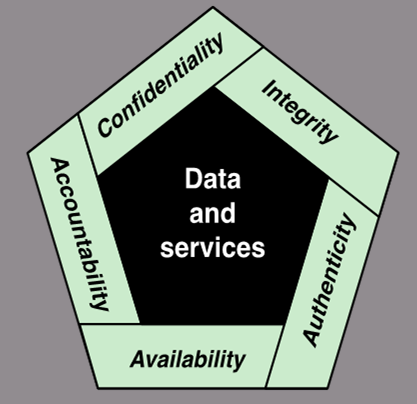
\includegraphics[width=8cm, keepaspectratio]{capitoli/cap_1/imgs/cia.png}
      \caption{Requisiti minimi per la Sicurezza Informatica.}
\end{figure}